%% Adaptado de 
%% http://www.ctan.org/tex-archive/macros/latex/contrib/IEEEtran/
%% Traduzido para o congresso de IC da USP
%%*****************************************************************************
% N�o modificar

\documentclass[onecolumn,conference,a4paper,11pt]{IEEEtran}

%******************************************************************************
% N�o modificar
\usepackage{IEEEtsup} % Defini��es complementares e modifica��es.
\usepackage[latin1]{inputenc} % Disponibiliza acentos.
\usepackage[english,brazil]{babel}
%% Disponibiliza Ingl�s e Portugu�s do Brasil.
\usepackage{latexsym,amsfonts,amssymb} % Disponibiliza fontes adicionais.
\usepackage{theorem} 
\usepackage[cmex10]{amsmath} % Pacote matem�tico b�sico 
\usepackage{url} 
%\usepackage[portuges,brazil,english]{babel}
\usepackage{graphicx}
\usepackage{amsmath}
\usepackage{amssymb}
\usepackage{color}
\usepackage[pagebackref=true,breaklinks=true,letterpaper=true,colorlinks,bookmarks=false]{hyperref}
\usepackage[tight,footnotesize]{subfigure} 
\usepackage[noadjust]{cite} % Disponibiliza melhorias em cita��es.
\usepackage[left=1cm,right=1cm,top=1cm,bottom=2cm]{geometry}
\newtheorem{definition}{Definition}
\newtheorem{thm}{Theorem}
%%*****************************************************************************

\begin{document}
\selectlanguage{english}
\renewcommand{\IEEEkeywordsname}{Palavras-chave}

%%*****************************************************************************

\urlstyle{tt}
% Indicar o nome do autor e o curso/n�vel (grad-mestrado-doutorado-especial)
\title{Cryptography in the Tor network}
\author{%
 \IEEEauthorblockN{Giovanni Bert�o \texttt{ra173325}\IEEEauthorrefmark{1}}
}

%%*****************************************************************************

\maketitle

%%*****************************************************************************
% Resumo do trabalho
\begin{abstract}
This essay presents how the Tor network applies cryptography
systems in order to implement the design of the onion routing
protocol and deploy a fully function network that allows anonymous
communication and is resistant against eavesdropping and traffic
analysis. Besides that, this essay presents the historical and
mathematical backgrounds need to understand the Tor network. And
for last it presents vulnerabilities and exploitations that target
Tor.
\end{abstract}

%%*****************************************************************************
% Modifique as se��es de acordo com o seu projeto

\section{Introduction}
One of the most concern about sending data through an insecure
channel is the possibility that the data can be read by someone
that was not meant to read it. Uncountable operations are done over
the internet these operations transports a lot of data every
second. However, the internet is an insecure channel, every data
can be a target of eavesdropping attack. Such attack, consists in someone to listen and
capture important data traffic over the internet.  The Tor network
similarly to any network is a set of computer and terminals
connected over the internet that implements the Onion routing
protocols~\cite{onion} to communicate. These protocols are based on
cryptographic operations applied in layers. Thus,
any message transported is protected against eavesdropping.
This essay is organized in the following way: Section~\ref{sec:hb}
describes historical facts and techniques that led to the current
implementation of Tor. Section~\ref{sec:mb} gives the main
mathematical results that are used into the design of Onion routing
protocols and later applied to Tor Network. Section~\ref{sec:ms}
main focus is on how the Tor network and the Onion
Protocols uses cryptographic algorithms and cryptographic implementations to
maintain anonymity of the users of Tor and to secure data against
sniffers. Furthermore, based on he previous sections, this essay will try to discuss some
cryptanalysis over Onion Routing protocols that led to possibles
attacks on the Tor network and section~\ref{sec:cc} presents the
concluding remarks and final comments.

\section{Historical Background}
\label{sec:hb}
This section will present how the onion routing protocols were
designed, what was their rationale and how cryptography achieved
it. After this, it will be presented how the Tor network, based on
the Onion routing protocol was implemented.

\subsection{Onion Routing Overview}
Nowadays, the internet is based on socket-connecting two machines
directly so they can exchange data and information. The onion
routing, instead, is based on stabilises a connection through a
sequence of machines. Those machines are know as \textit{onion
routers}. The onion routing maintains a set of properties:
\begin{itemize}
\item The onion routing must relay on a decentralized network;
\item This network consists in a set of onion routers;
\item The data is send through a sequence of onion routers from the
initiator to the receiver;
\item The route that the data will flow is defined at the network
setup time;
\item The data must be different each time it pass through a
router.
\end{itemize}
Based on those properties it's possible to maintain a
anonymous connection between the initiator and the responder.
Because, anyone eavesdropping the communication will not know who
are the initiator and the receiver since the data must travel
through a set network of machines. Since the data is different in
each router, the data cannot be tracked.

\subsection{TOR network Overview}
During the 90s the Internet lacks of security so it was clear the
possibility of surveillance and tracking over the internet. In
1995, David Goldschlag, Mike Reed, and Paul Syverson at the U.S.
Naval Research Lab (NRL) deployed the prototype of the onion
routing protocol~\cite{onion}. Which the goal was to increase the
privacy while using the Internet. In the early 2000s Roger
Dingledine, a recent Massachusetts Institute of Technology (MIT),
based on the onion routing protocol started the TOR project, later
on the project was deployed to use~\cite{tor}.

\subsection{How TOR was implemented based on the onion routing
protocol}
Based on the properties of the onion routing protocol TOR attempts
to anonymize the transport layer in the following way:
\begin{itemize}
\item First, the client software gets a list of Tor nodes;
\item Then, The software incrementally creates a private pathway ---
know as Tor circuit --- across the network via encrypted
connections;
\item Once the circuit is chosen, the client tunnels the circuit
nodes in a way that each node just know the immediately preceding
and following nodes;
\item The data is sent from the source Tor node to the destination
Tor node through the circuit;
\item For each node through the Tor circuit, the data is encrypted;
\end{itemize}
Those steps are related to onion routing properties. The first and
second ones are related to the
decentralized network via onion routers. Limiting the knowledge of
each node to just the immediately following node prevents
individuals nodes to know the complete path grants anonymity of the
source and the destination. The non-tracking
policy of the onion routing protocol applies to the data over Tor,
since the data is encrypted in each node the data is going to be
different in each node.

\subsection{Tor Network Cryptography}
The Tor network implements a set of cipher
algorithms~\footnote{https://gitweb.torproject.org/torspec.git/tree/tor-spec.txt}.
\begin{itemize}
\item Stream cipher: 128-bit AES;
\item Public-key cipher: RSA 1024-bit and fixed exponent of 65537,
OAEP-MGF1 padding with SHA-1 digest function;
\item Signature: Curve25519 and Ed25519;
\item Key-Exchange: Diffie-Hellman with generator (g) of 2. For
modulus (p), they use 1024-bit safe prime from rfc2409 (Internet
Key Exchange);
\item HashFunction: SHA-1;
\end{itemize}

\section{Mathematical Background}
\label{sec:mb}
This section will discuss the mathematical background of the
cryptographic operations presented on the previous section.

\subsection{Galois Field}
In AES, Galois field arithmetic is used in most layers, especially
in the S-Box and the MixColumn layer. A finite field, sometimes
also called Galois field, is a set with a finite number of
elements. The following definitions and theorems are the
mathematical base for almost every cryptosystem~\cite{livro}.
\begin{definition}{Group}
A group is a set of elements $G$ together with an operation $\circ$ which
combines two elements of $G$. A group has the following properties:
\begin{enumerate}
\item The group operation $\circ$ is closed. That is, $\forall a,
b, \in G$, it holds that $a \circ b = c \in G$.
\item The group operation is associative. That is, $a\circ (b\circ
c) = (a \circ b)\circ c$ $\forall a, b, c \in G$.
\item There is an element $1 \in G$, called the neutral element (or
identity
element), such that $a \circ 1 = 1 \circ a = a$ $\forall a \in G$.
\item For each $a \in G$ there exists an element $a^{-1} \in G$,
called the inverse of $a$, such that $a \circ a^{-1} = a^{-1} \circ
a = 1$.
\item A group $G$ is abelian (or commutative) if, furthermore, $a \circ b =
b \circ a$ $\forall a, b \in G$.
\end{enumerate}
\end{definition}

\begin{definition}{Field}
A field $F$ is a set of elements with the following properties:
\begin{itemize}
\item All elements of $F$ form an additive group with the group
operation "+" and the neutral element 0.
\item All elements of $F$ except 0 form a multiplicative group with the
group operation "x" and the neutral element 1.
\item When the two group operations are mixed, the distributivity law
holds, i.e., $\forall a, b, c \in F \to a(b + c) = (ab) + (ac)$.
\end{itemize}
\end{definition}

\begin{thm}
A field with order m only exists if $m$ is a prime power, i.e., $m
= p^n$ , for some positive integer $n$ and prime integer $p$. $p$
is called the characteristic of the finite field.
\end{thm}

\begin{thm}
Let $p$ be a prime. The integer ring $\mathbb{Z}_p$ is denoted
as $GF(p)$ and is referred to as a prime field, or as a Galois field
with a prime number of elements. All nonzero elements of $GF(p)$
have an inverse. Arithmetic in $GF(p)$ is done modulo $p$.
\end{thm}
\subsection{AES}
The AES is a well-know block cipher which operates in blocks of
size of 128-bits. An overview of the input/output parameters can be
seen in the Figure~\ref{fig:aes}. The AES consists in layers
operations each layer manipulates the entire block. The layers are
described in most of the cryptography textbooks~\cite{livro}. The
algorithm apply the layers in rounds, using a key of 128 bits means
that 10 rounds will be applied.
\begin{figure}
\centering
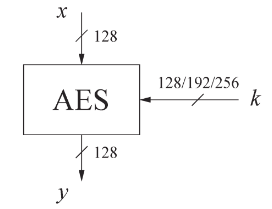
\includegraphics[width=0.5\textwidth]{figuras/aes.png}
\caption{Basic AES input/output representation.}
Source:~\cite{livro}.
\label{fig:aes}
\end{figure}
\begin{itemize}
\item Key Addition Layer: A 128-bit round key, or subkey, which has
been derived from the main key in the key schedule, is XORed to the
state.
\item Byte Substitution layer (S-Box): Each element of the state is
nonlinearly transformed using lookup tables with special
mathematical properties.  This introduces confusion to the data,
i.e., it assures that changes in individual state bits propagate
quickly across the data path.
\item Diffusion Layer: It provides diffusion over all state bits.
It consists of two sublayers, both of which perform linear
operations:
\begin{itemize}
\item The ShiftRows Layer: permutes the data on a byte level.
\item The MixColumn Layer: is a matrix operation which combines
(mixes) blocks of four bytes.
\end{itemize}
\end{itemize}

\subsection{RSA}
The RSA(Rivest-Shamir-Adleman) is a well-know public-key algorithm
of asymmetric key. The underlying one-function is based on the
Integer Factorization problem. Encryption and Decryption uses the
same function. Given the public key ($n,e$) = $k_{pub}$ and the
plaintext $x$, the encryption function is presented in
Equation~\ref{eq:enc}. Given the private key $d$ = $k_{pr}$ and
the ciphertext $y$, the decryption function is presented in
Equation~\ref{eq:dec}.
\begin{equation}
\label{eq:enc}
y = e_{k_{pub}}(x) = x^e mod n
\end{equation}
\begin{equation}
\label{eq:dec}
x = e_{k_{pr}}(y) = y^d mod n
\end{equation}


\subsection{Curve25519}
Elliptic Curves is based on the generalized discrete logarithm
problem. 
\begin{definition}
Discrete Logarithm Problem: given a group G, a generator g of the group and an element h of G,
find the discrete logarithm to the base g of h in the group G.
\end{definition}
Curve25519, a state-of-the-art elliptic-curveDiffie-Hellman
function suitable for a wide variety of cryptographic applications.
This paper uses Curve25519 to obtain new speed records for
high-security DiffieHellman computations. Each Curve25519 user has
a 32-byte secret key and a 32-byte public key. Each set of two
Curve25519 users has a 32-byte shared secret used to authenticate
and encrypt messages between the two users~\cite{curve}.

\subsection{Ed25519}
The Edwards-curve Digital Signature Algorithm (EdDSA) is a variant
of Schnorr's signature system with (possibly twisted) Edwards
curves.  EdDSA needs to be instantiated with certain parameters,
and this document describes some recommended
variants~\footnote{https://tools.ietf.org/html/rfc8032}. The
Ed25519 is the EdDSA signature scheme using SHA-512 and the
Curve25519.  Specifically, Ed25519-SHA-512 is EdDSA with the
following parameters: $b$ = $256$; H is SHA-512; $q$ is the prime
$2^{255}-19$; the 255-bit encoding of $F_{2^{255}-19}$ is the
usual little-endian encoding of \{0, 1, ..., $2^{255}-20$\}; $l$ is
the prime $2^{252}+27742317777372353535851937790883648493$
from~\cite{curve}; $d = -121665/121666 \in F_q$; and B is the
unique point $(x, 4/5) \in$ E for which $x$ is
positive~\cite{ed25519}.

\subsection{Diffie-Hellman Key Exchange}
The Diffie-Hellman key exchange (DHKE), proposed by Whitfield
Diffie and Martin Hellman in 1976~\cite{dh}, was the first
asymmetric scheme published in the open literature~\cite{livro}.
The basic idea behind the DHKE is that exponentiation in $Z^*_p$ ,
$p$
prime, is a
one-way function and that exponentiation is commutative, i.e.,
$k = (\alpha ^x)^y \equiv (\alpha^y)^x$ mod $p$. The value $k =
(\alpha ^x)^y \equiv (\alpha^y)^x$ mod $p$ is the joint secret which
can be used as the session key between the two parties.

The set-up protocol consists of the following steps:
\begin{definition}{Diffie-Hellman Set-up}
\begin{enumerate}
\item Choose a large prime $p$;
\item Choose an integer $\alpha \in \{2,3,...,p-2\}$;
\item Publish $p$ and $\alpha$.
\end{enumerate}
\end{definition}

Once the set-up is completed and we can move to the Key Exchange
procedure as show in Figure~\ref{fig:dhke}.

\begin{figure}
\centering
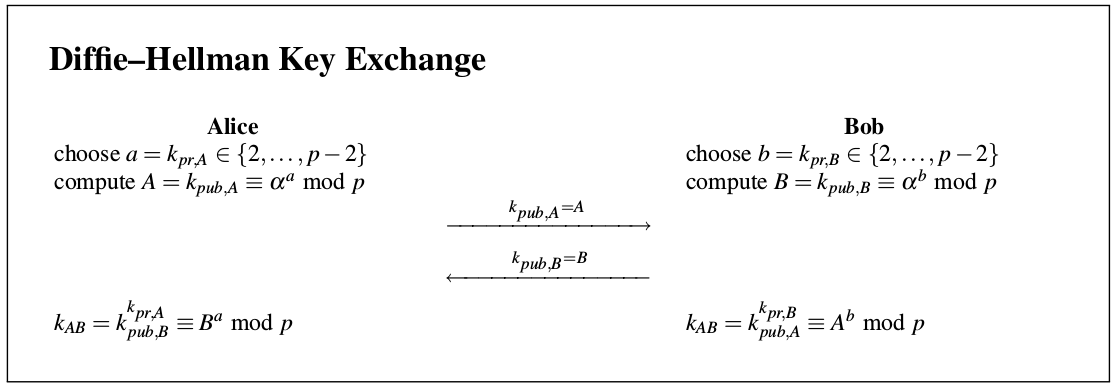
\includegraphics[width=\textwidth]{figuras/dhke.png}
\caption{Diffie-Hellman Key Exchange procedure.}
Source:~\cite{livro}.
\label{fig:dhke}
\end{figure}

\subsection{RFC 2409 - Internet Key Exchange}
Hybrid protocol based on ISAKMP~\cite{isakmp}, Oakley~\cite{oakley}
and SKEME~\cite{skeme}. The propose of
this protocol is to negotiate, and provide authenticated keying
material for, security associations in a protected
manner~\footnote{https://tools.ietf.org/html/rfc2409}.

\subsection{TLS/SSL}
The primary goal of the TLS Protocol is to provide privacy and data
integrity between two communicating applications. The protocol is
composed of two layers: the TLS Record Protocol and the TLS
Handshake Protocol. At the lowest level, layered on top of some
reliable transport protocol (e.g., TCP), is the TLS Record
Protocol. The TLS Record Protocol provides connection security that
has two basic
properties~\footnote{https://tools.ietf.org/html/rfc2246}:
\begin{itemize}
\item  The connection is private. Symmetric cryptography is used
for data encryption (e.g., DES) The keys for
this symmetric encryption are generated uniquely for each
connection and are based on a secret negotiated by another protocol
\item The connection is reliable. Message transport includes a
message integrity check using a keyed MAC. Secure hash functions
(e.g., SHA, MD5, etc.) are used for MAC computations.
\end{itemize}
The TLS Handshake Protocol, allows the server and client to
authenticate each other and to negotiate an encryption algorithm
and cryptographic keys before the application protocol transmits or
receives its first byte of data. The TLS Handshake Protocol
provides connection security that has three basic properties:
\begin{itemize}
\item The peer's identity can be authenticated using asymmetric, or
public key, cryptography (e.g., RSA [RSA]).
\item The negotiation of a shared secret is secure: the negotiated
secret is unavailable to eavesdroppers, and for any authenticated
connection the secret cannot be obtained, even by an attacker who
can place himself in the middle of the connection.
\item  The negotiation is reliable: no attacker can modify the
negotiation communication without being detected by the parties to
the communication.
\end{itemize}

SSL is the predecessor of TLS. The SSL protocol consists of two
phases: handshake and data transfer. During the handshake phase,
the client and server use a public-key encryption algorithm to
determine secret-key parameters. During the data transfer phase,
both sides use the secret key to encrypt and decrypt successive
data transmissions.  The client initiates an SSL handshake
connection by first transmitting a Hello message.This message
contains a list of the secret-key algorithms, called cipher specs,
that the client supports. The server responds with a similar Hello
message, selecting its preferred cipher spec. Following the Hello
message, the server sends a certificate that contains its public
key. Allowing the possibility to stablish an secure connection
between client and server. Although the SSL protocol was found to
be insecure and was substituted by the TLS protocol~\cite{ssl}.

\section{Main Section}
\label{sec:ms}
This section will describe how the cryptographic functions and how
the mathematical background were used when the onion routing
protocols were designed. Furthermore, it will show how the Tor
network implements this design. At least, this section will discuss how
attacks, exploitations and possible counter-measures over the Tor network cryptography and
architecture.

\subsection{How Tor network implements cryptography}
\subsubsection{Assigning keys to relays}
Tor relays are nothing more than onion routers. Which are each
machine on the Tor network. So, to allow any crypto system over the
network those machines must have a key pair of public and private
key~\footnote{https://gitweb.torproject.org/torspec.git/tree/tor-spec.txt}. Thus, every single Tor relay has multiple public/private
keypairs:

\begin{itemize}
\item These are 1024-bit RSA keys:
\begin{itemize}
\item A long-term signing-only "Identity key" used to sign
documents and certificates, and used to establish relay identity.
\item A medium-term TAP "Onion key" used to decrypt onion skins
when accepting circuit extend attempts.
\item A short-term "Connection key" used to negotiate TLS
connections.
\end{itemize}
\item This is Curve25519 key:
\begin{itemize}
\item A medium-term ntor "Onion key" used to handle onion key
handshakes when accepting incoming circuit extend requests.
\end{itemize}
\item These are Ed25519 keys:
\begin{itemize}
\item A long-term "master identity" key.  This key never changes;
it is used only to sign the "signing" key below.  It may be kept
offline.
\item A medium-term "signing" key.  This key is signed by the
master identity key, and must be kept online.  A new one should be
generated periodically.  It signs nearly everything else.
\item A short-term "link authentication" key, used to authenticate
the link handshake: see section 4 below.  This key is signed by the
"signing" key, and should be regenerated frequently.
\end{itemize}
\end{itemize}

\subsubsection{Establishing a Connection}
Connections between two Tor relays, or between a client and a
relay, use TLS/SSLv3 for link authentication and encryption.  All
implementations MUST support the SSLv3 ciphersuite
"TLS\_DHE\_RSA\_WITH\_AES\_128\_CBC\_SHA" if it is available~\footnote{https://gitweb.torproject.org/torspec.git/tree/tor-spec.txt}.

\subsubsection{Creating a Circuit}
When creating a cricuit through the network, the circuit creator
(OP) performs the following
steps~\footnote{https://gitweb.torproject.org/torspec.git/tree/tor-spec.txt}:
\begin{enumerate}
\item Choose an onion router as an end node $R_n$, $n >= 3$ to
grant an anonymous connection;
\item Choose a chain of $(n-1)$ onion routers
$(R_1,...,R_{n-1})$ such that no router appears twice, i.e. the
chain = $\{R_1,...,R_{n-1}\ : \text{For } i,j \text{ such that }1 \le i < j \le n-1, R_i
\not= R_j\}$.
\item If not already connected to the first router in the chain,
open a new connection to that router.
\item Choose a circuit ID not already in use on the connection with the
first router in the chain; send a CREATE/CREATE2 cell --- The
traffic flowing into the circuit is sent in fixed-size "cells",
Figure~\ref{fig:cell} shows a generic cell architecture ---
along the connection, to be received by the first onion router.
\item Wait until a CREATED/CREATED2 cell is received; finish the
handshake and extract the forward key $Kf_1$ and the backward key
$Kb_1$.
\item For each subsequent onion router $R$ ($R_2$ through $R_n$),
extend the circuit to $R$.
\end{enumerate}
To extend the circuit by a single onion router $R_M$, the OP performs
these steps:
\begin{enumerate}
\item Create an onion skin --- Encrypted data --- encrypted to
$R_M$'s public onion key.
\item Send the onion skin in a relay EXTEND/EXTEND2 cell along
the circuit.
\item When a relay EXTENDED/EXTENDED2 cell is received, verify
$KH$ --- the handshake key --- and calculate the shared keys.  The
circuit is now extended.
\end{enumerate}

\begin{figure}
\centering
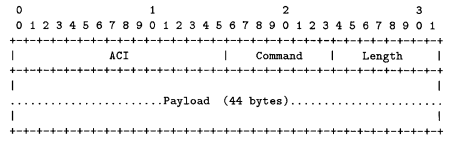
\includegraphics[width=\textwidth]{figuras/cell.png}
\caption{Generic cell.}
Source:~\cite{onion}.
\label{fig:cell}
\end{figure}

\subsubsection{How do data flow over Tor network}
Data moves through an anonymous connection in DATA
cells. At each onion router both the length and payload fields of
a cell are crypted using the appropriate cryptographic engine.
The new cell is sent out to the appropriate neighbor. The
onion proxy must repeatedly crypt data to either add the
appropriate layers of cryption on outgoing data, or remove
layers of cryption from incoming data. When constructing a
DATA cell from a plaintext data stream, the cell is (partially)
filled, its true length is set, and all 45 bytes of the length and
payload fields are repeatedly crypted using the stream ciphers
defined by the onion. Therefore, when the cell arrives at the
exit funnel, the length field reflects the length of the actual
data carried in the payload.~\cite{onion}.
Therefore, for each router the data is encrypted in a
layered-fashion as shown in Figure~\ref{fig:data}. Thus, each node
cannot decrypt the previous node encryption.

\subsubsection{How to access sites over the Tor network}
Suppose Alice wants to access Bob site over the Tor network. The
major goal is to stablish an circuit from Alice to Bob. For this
the first step is: Alice must obtain a Tor node list as show in
Figure~\ref{fig:step1}. Once Alice gather the Tor node list, a
circuit will be constructed in a random fashion using the previous
detailed algorithm, this is step is illustrated by
Figure~\ref{fig:step2}. Now, Alice has a circuit with an entry node
being at the first row and first column and the exit node being at
the last row and last column. Thus, data can be sent from Alice to
Bob and gather from Bob to Alice. Therefore, suppose Alice wants to
access Jane's site now. A new circuit is needed to prevent people
linking Alice actions to former circuits. So, to access Jane's site
Alice recreates a new circuit as shown in Figure~\ref{fig:step3}.

\begin{figure}
\centering
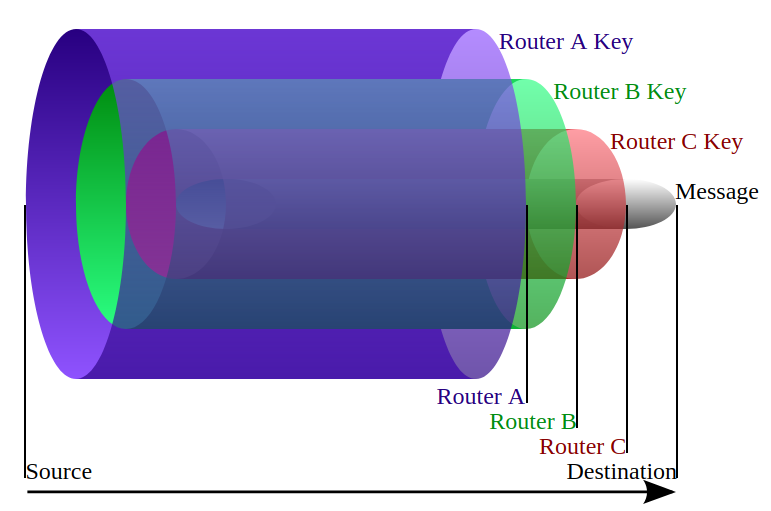
\includegraphics[width=0.5\textwidth]{figuras/data.png}
\caption{Data encryption.}
Source: https://en.wikipedia.org/wiki/File:Onion\_diagram.svg
\label{fig:data}
\end{figure}

\begin{figure}
\centering
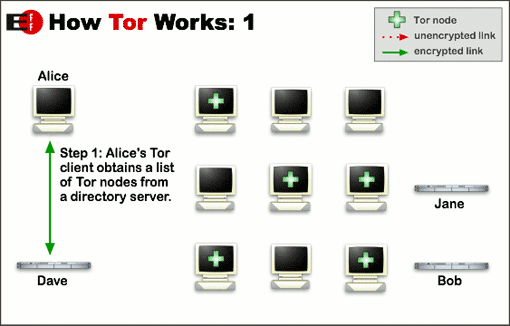
\includegraphics[width=\textwidth]{figuras/step1.png}
\caption{First step: Gather the Tor nodes list.}
Source:https://2019.www.torproject.org/about/overview.
\label{fig:step1}
\end{figure}

\begin{figure}
\centering
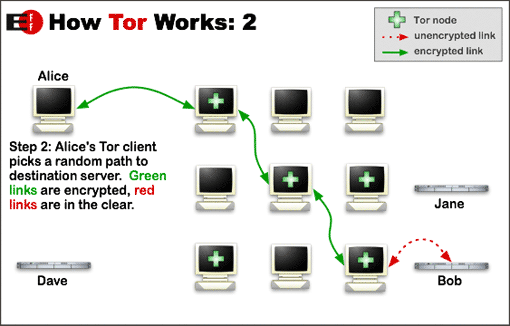
\includegraphics[width=\textwidth]{figuras/step2.png}
\caption{The circuit from Alice to Bob is formed. Note which
connections are encrypted.}
Source:https://2019.www.torproject.org/about/overview.
\label{fig:step2}
\end{figure}

\begin{figure}
\centering
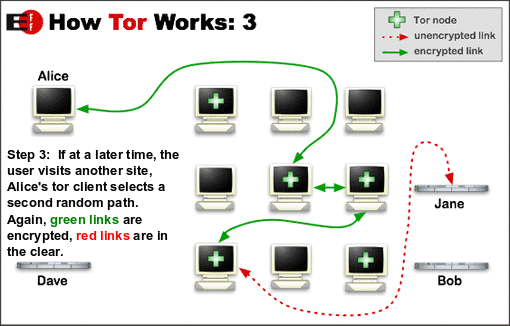
\includegraphics[width=\textwidth]{figuras/step3.png}
\caption{If Alice wants to access another site a new circuit will
be needed.}
Source:https://2019.www.torproject.org/about/overview.
\label{fig:step3}
\end{figure}

\subsubsection{Hidden Services and Rendezvous Points}
Tor allows users to hide theirs locations by establishing a
rendezvous point and an introduction point. An onion service needs to
advertise its existence in the Tor network before clients will be
able to contact it. To accomplish this an onion service randomly
pick an router, build a circuit to them and gives his public-key so
it can acts as a introduction point. Since the introduction point
is not on the service location and it only has the public-key of
the onion service it's hard to anyone associate the
introduction point to a service IP address or its
location~\cite{tor2}.
As example, suppose Bob wants to deploy a onion hidden service and
Alice wants to access it. The following steps shows how Bob can
achieve it:
\begin{itemize}
\item The first step consists on Bob randomly
select a set of routers that will be used as introductions points,
as shown in Figure~\ref{fig:h1};
\item Once the introduction points were selected, Bob assembles an
onion service descriptor containing his public-key;
\item Then, Bob sends to a distributed hash table the descriptor
and a summary of each introduction point, as shown in
Figure~\ref{fig:h2};
\item The client (Alice) wants to access the hidden service
deployed by Bob. So, first Alice needs to learn about the service;
\item Alice contacts the hash table to learn about the service and
acquire the descriptors and the summary of each introduction point;
\item Alice contacts a router and asks it to act as a rendezvous
point, as shown in Figure~\ref{fig:h3};
\item When the rendezvous point is ready, Alice sets-up an
introduction message including the rendezvous address;
\item Alice sends this message to an introduction point requesting
to be delivered to the onion service, as shown in
Figure~\ref{fig:h4};
\item Bob receives and decrypts the introduction message, finding
the rendezvous address. Allowing, Bob to stablish a circuit to the
rendezvous point, as shown in Figure~\ref{fig:h5}.
\item Once the circuit is on, Alice receives a notification about
the successful connection establishment;
\item Now, both Alice and Bob can use their circuit to the
rendezvous point to communicate between them, as shown in
Figure~\ref{fig:h6}.
\end{itemize}

\begin{figure}
\centering
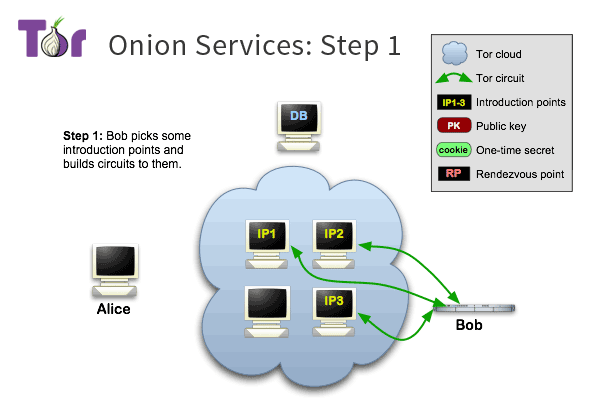
\includegraphics[width=0.8\textwidth]{figuras/h1.png}
\caption{First step on hidden service deploy. Bob picks the
introduction points.}
Source: {https://2019.www.torproject.org/docs/onion-services}.
\label{fig:h1}
\end{figure}

\begin{figure}
\centering
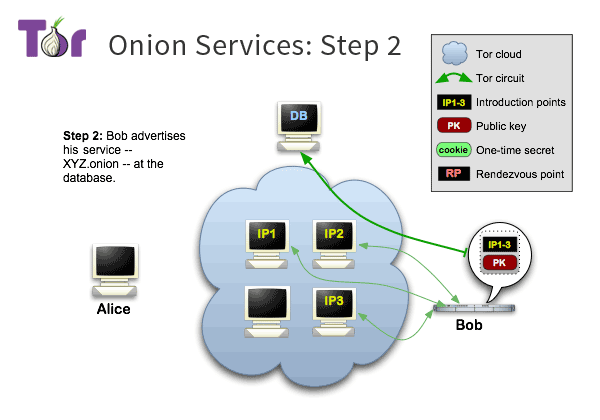
\includegraphics[width=0.8\textwidth]{figuras/h2.png}
\caption{Bob stores a descriptor and a summary of the hidden
service in a hash distributed table}
Source: {https://2019.www.torproject.org/docs/onion-services}.
\label{fig:h2}
\end{figure}

\begin{figure}
\centering
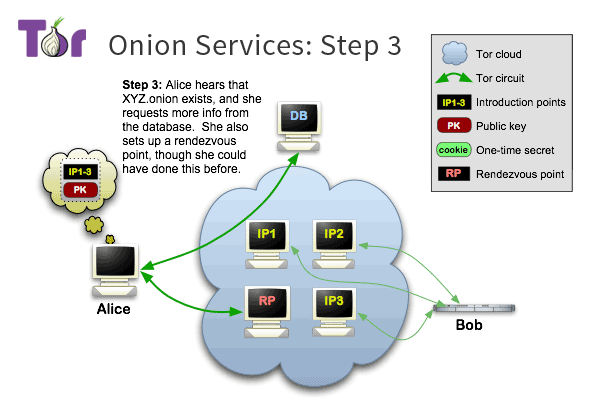
\includegraphics[width=0.8\textwidth]{figuras/h3.png}
\caption{Alice retrieves information of the hidden service from the
table and pick a router to act as a rendezvous point.}
Source: {https://2019.www.torproject.org/docs/onion-services}.
\label{fig:h3}
\end{figure}

\begin{figure}
\centering
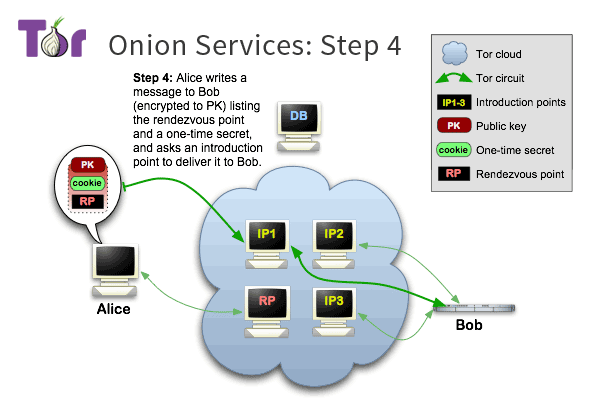
\includegraphics[width=0.8\textwidth]{figuras/h4.png}
\caption{Alice sets-up an introduction message containing a
one-time secret and the rendezvous address.}
Source: {https://2019.www.torproject.org/docs/onion-services}.
\label{fig:h4}
\end{figure}

\begin{figure}
\centering
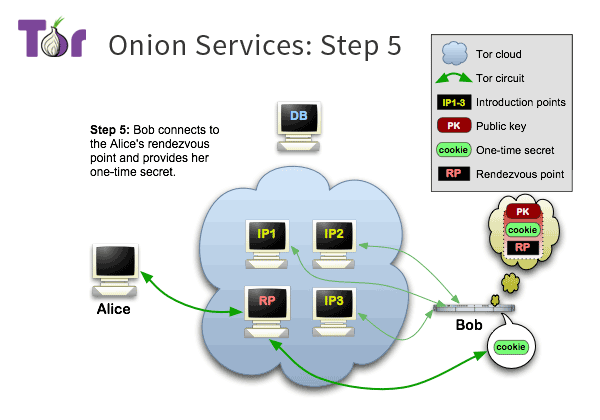
\includegraphics[width=0.8\textwidth]{figuras/h5.png}
\caption{Bob decrypts the message and sets-up a connection to the
rendezvous point. Once the connection was successfully established,
Alice receives a notification.}
Source: {https://2019.www.torproject.org/docs/onion-services}.
\label{fig:h5}
\end{figure}

\begin{figure}
\centering
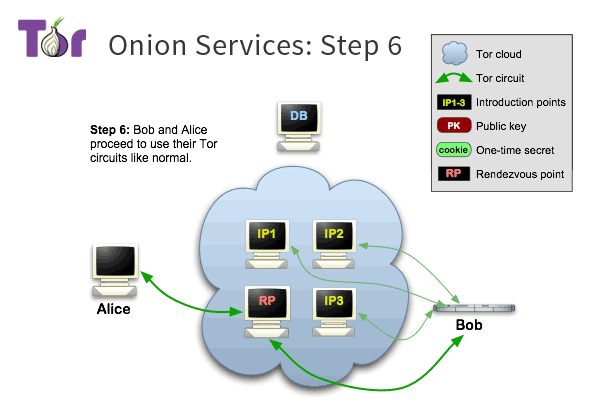
\includegraphics[width=0.8\textwidth]{figuras/h6.png}
\caption{Bob and Alice can communicate via the rendezvous point. The
rendezvous just pass the message and acts as a end-to-end
messenger}
Source: {https://2019.www.torproject.org/docs/onion-services}.
\label{fig:h6}
\end{figure}

\subsection{Attacks on Tor network}
Besides the well-known cryptanalysis techniques that can be
deployed over the crypto-systems used by Tor. There is a set of
attacks that targets the Tor architecture.

\subsubsection{Tagging-Attack}
Based on the design of the onion protocol there is the following
attacks known as the Tagging attack: If Oscar controls both
the first(entry) and the last(exit) nodes picked by Alice when
trying to connect Bob. Oscar can modify the data on the
entry-point("Tagging it"), and detect the modification at the exit
point. Thus, Oscar can confirm that it is really Alice talking to
Bob. But, since this attack involve modifying the data that could
drop the connection, this attack is limited. Therefore, there is an
passive variant of this attack that can be performed by an observer
like an ISP. Counter-measure: The Tor design and the onion routing
protocol design does not implement an
counter-measure for the Tagging-Attack~\cite{tor2}.

\subsubsection{Run an onion proxy}
It is expected that end users will nearly
always run their own local onion proxy. However, in some
settings, it may be necessary for the proxy to run remotely-typically, in institutions that want to monitor the activity of
those connecting to the proxy. Compromising an onion proxy
compromises all future connections through it. Counter-measure:
Identify such malicious routers and blacklist them~\cite{tor2}.

\subsubsection{Run a hostile OR}
In addition to being a local observer, an isolated hostile node can
create circuits through itself, or alter traffic patterns to affect
traffic at other nodes. Nonetheless, a hostile node must be
immediately adjacent to both endpoints to compromise the anonymity
of a circuit. If an adversary can run multiple routers, and can
persuade the directory servers that those routers are trustworthy
and independent, then occasionally some user will choose one of
those routers for the start and another as the end of a circuit. If
an adversary controls $m > 1$ of $N$ nodes, he can correlate at
most $(\dfrac{m}{N})^2$ of the traffic --- although an adversary
could still attract a disproportionately large amount of traffic by
running an OR with a permissive exit policy, or by degrading the
reliability of other routers. Counter-measure: Identify such
malicious routers and blacklist them~\cite{tor2}.

\subsubsection{Distribute hostile code}
An attacker could trick user into running subverted Tor software
that did not, in fact, anonymize their connections or worse, could
trick routers into running weakened software that provided users
with less anonymity. Counter-measure: all Tor releases are in
source code form and warn users to never trust any software that
comes without source~\cite{tor2}.

\subsubsection{Timing attack}
Since Tor is a low latency anonymity system, the Tor network is
susceptible target for timing attack. Such attack consists in
analyze the time taken to execute cryptographic algorithms. 
Murdoch and Danezis~\cite{time} describe an attack that allows a
single malicious Tor server and a colluding Web server (or other
service provider), to identify all three nodes of a Tor circuit
used by a client for a given session (ideally, only the exit node's
identity should be known to the service provider).  However, this
system does not identify the client directly, only its entry node
into the Tor network. The attack works as follows: When a client
connects to the malicious Web server, that server modulates its
data transmission back to the client in such a way as to make the
traffic pattern easily identifiable by an observer. At least one
Tor server controlled by the adversary builds "timing" circuits
through each Tor server in the network. These circuits all have
length one, beginning and terminating at the adversarial Tor node.
By sending traffic through timing circuits to measure latency, the
adversary is able to detect which Tor servers process traffic that
exhibits a pattern like that which the attacker Web server is
generating.  Since Tor does not reserve bandwidth for each
connection, when one connection through a node is heavily loaded,
all others experience an increase in latency.  By determining which
nodes in the Tor network exhibit the server-generated traffic
pattern, the adversary can map the entire Tor circuit used by the
client. Counter-measure: Identify and blacklist such nodes~\cite{leak}.

\subsubsection{Attack on Randevouz points}
The known randevouz points attacks mainly consists in DoS attacks.
The counter-measures consists in analysing the data traffic through
the introduction point and detect any attempt of DoS attack. Beside
this, the introduction points are no different from a onion router,
so the same attacks that target onion routers can target randevouz
points~\cite{tor2}.

\subsubsection{Tor Censorship --- Directory Attacks}
This is not a cryptanalysis attack, it simply consists in an
attempt to incapacitate the network through the seizure of
specialized servers in the network called directory authorities.
Such directories retrieve the list of routers to a Tor
client. Thus, without the nodes there is no circuit and there is no
network~\footnote{https://blog.torproject.org/possible-upcoming-attempts-disable-tor-network}.

\section{Closing Comments}
\label{sec:cc}
This essay describes how the Tor network applies cryptographic
systems to implement the onion routing protocol that allows an
anonymous connection to be established. Such connections are
resistant to traffic analysis and eavesdropping. Those connection
allow two onion routers to communicate between them without
reveling details about the connection. Because, the onion routing
moves the anonymity of the communication infrastructure to below
the application layer, trying to secure the transport layer. Based
on this, the onion routing protocol is used as a primitive on
anonymous communication protocol.Tor network uses cryptographic
operations and protocol to apply those primitives implementing a
working anonymous network. Such network is used today by the entire
world with the main goals of maintain the privacy over a insecure
channel like the internet. The Tor network achieves it main goals
based on their characteristic of deployability, usability and
simple design. Besides the security of the cryptographic
algorithms, the Thor network have some questions before it can be
entirely trusted. Such as, how long a circuit must be; Tor network
can be a target of end-to-end attack since it is based on the
design of the onion routing protocol and is a low-latency system;
The security of the network depends on the number of the users,
number of routers, number of servers and who owns the majority of
onion routers on the network.

%******************************************************************************
% Refer�ncias - Definidas no arquivo Relatorio.bib

\bibliographystyle{IEEEtran}

\bibliography{Relatorio}
\label{sec:cc}


%******************************************************************************
\end{document}
